%==============================================================================
% Sjabloon onderzoeksvoorstel bachelorproef
%==============================================================================
% Gebaseerd op LaTeX-sjabloon ‘Stylish Article’ (zie voorstel.cls)
% Auteur: Jens Buysse, Bert Van Vreckem

% TODO: Compileren document:
% 1) Vervang ‘naam_voornaam’ in de bestandsnaam door je eigen naam, bv.
%    buysse_jens_voorstel.tex
% 2) pdflatex naam_voornaam_voorstel.tex (2 keer)
% 3) biber naam_voornaam_voorstel
% 4) pdflatex naam_voornaam_voorstel.tex (1 keer)

\documentclass[fleqn,10pt]{voorstel}
\usepackage{pgfplots}

%------------------------------------------------------------------------------
% Metadata over het artikel
%------------------------------------------------------------------------------

\JournalInfo{HoGent Bedrijf en Organisatie}
\Archive{Bachelorproef 2016 - 2017}

%---------- Titel & auteur ----------------------------------------------------

% TODO: geef werktitel van je eigen voorstel op
\PaperTitle{Tracing in microservices met Spring Cloud Sleuth en Zipkin}
\PaperType{Onderzoeksvoorstel Bachelorproef} % Type document

% TODO: vul je eigen naam in als auteur, geef ook je emailadres mee!
% TODO: vul de naam van je co-promotor(en) in als tweede (derde, ...) auteur.
% Dien je voorstel pas in nadat je co-promotor de kans gehad heeft na te lezen
% en feedback te geven!
\Authors{Frederic Everaert\textsuperscript{1}, Geert Vandensteen\textsuperscript{2}} % Authors
\affiliation{\textbf{Contact:}
  \textsuperscript{1} \href{mailto:frederic.everaert.u1028@student.hogent.be}{frederic.everaert.u1028@student.hogent.be};
  \textsuperscript{2} \href{mailto:geert.vandensteen@synthetron.com}{geert.vandensteen@synthetron.com}}

%---------- Abstract ----------------------------------------------------------

\Abstract{
Microservices worden steeds populairder t.o.v. monolithische applicaties. De voordelen ervan worden vaak genoemd, maar een nadeel, dat vaak genegeerd wordt, is dat het opzetten van microservices complex kan zijn doordat requests verschillende onafhankelijke services doorkruisen. Gewone debugging tools zijn dan niet meer voldoende en een oplossing is nodig om de complexiteit te beantwoorden. Deze bachelorproef onderzoekt hoezeer tracing een oplossing is voor dit probleem. Specifiek Spring Cloud Sleuth en Zipkin worden onder de loep genomen waarbij de verschillende microservices opgezet worden met Docker. De verwachting is dat tracing een onmisbare tool is voor microservices en er hiervoor alleen maar meer en betere tools en oplossingen bedacht zullen worden in de toekomst.
}

%---------- Onderzoeksdomein en sleutelwoorden --------------------------------
% TODO: Sleutelwoorden:
%
% Het eerste sleutelwoord beschrijft het onderzoeksdomein. Je kan kiezen uit
% deze lijst:
%
% - Mobiele applicatieontwikkeling
% - Webapplicatieontwikkeling
% - Applicatieontwikkeling (andere)
% - Systeem- en netwerkbeheer
% - Mainframe
% - E-business
% - Databanken en big data
% - Machine learning en kunstmatige intelligentie
% - Andere (specifieer)
%
% De andere sleutelwoorden zijn vrij te kiezen

\Keywords{Applicatieontwikkeling. Microservices --- Tracing --- Debugging} % Keywords
\newcommand{\keywordname}{Sleutelwoorden} % Defines the keywords heading name

%---------- Titel, inhoud -----------------------------------------------------
\begin{document}

\flushbottom % Makes all text pages the same height
\maketitle % Print the title and abstract box
\tableofcontents % Print the contents section
\thispagestyle{empty} % Removes page numbering from the first page

%------------------------------------------------------------------------------
% Hoofdtekst
%------------------------------------------------------------------------------

%---------- Inleiding ---------------------------------------------------------

\section{Introductie} % The \section*{} command stops section numbering
\label{sec:introductie}
%
%Hier introduceer je werk. Je hoeft hier nog niet te technisch te gaan.
%
%Je beschrijft zeker:
%
%\begin{itemize}
%  \item de probleemstelling en context
%  \item de motivatie en relevantie voor het onderzoek
%  \item de doelstelling en onderzoeksvraag/-vragen
%\end{itemize}

Monolithische architecturen ruimen steeds meer baan voor microservice architecturen of kortweg microservices. Een monolitische applicatie is gebouwd als een enkelvoudige, zelfstandige eeheid. Bij een client-server model, kan bijvoorbeeld de applicatie langs de server zijde bestaan uit een enkele applicatie die de HTTP requests behandelt, logica uitvoert en data ophaalt of bijwerkt in de database. Het grote probleem van monolitische applicaties is dat ze moeilijk te onderhouden zijn. Een kleine verandering in een bepaalde functionaliteit van de applicatie kan ervoor zorgen dat andere delen van de applicatie ook bijgewerkt moeten worden. De volledige applicatie moet opnieuw gebuild en gedeployed worden. Als een bepaalde functionaliteit gescaled moet worden, moet de volledige applicatie gescaled worden. Microservices bieden hiervoor een oplossing, aangezien de verschillende functionaliteiten elk een op zich zelf staande service kunnen vormen. \\

Bij microservices schieten echter de traditionele tools voor debugging tekort. Een enkele service kan niet het volledige beeld geven over bijvoorbeeld de performantie van de applicatie in zijn geheel. Om dit te verhelpen, kunnen requests getraced worden. Een trace is de volledige reisweg van een request die spans bevat voor alle doorkruiste microservices. Een span bestaat uit tags of metadata zoals de start- en stoptijdstippen. Deze data kan dan verzameld worden om een volledig beeld van het gedrag van de applicatie te geven. \\

De bedoeling van dit onderzoek is om de meerwaarde van tracing in microservices aan te tonen en ook om eventuele tekortkomingen vast te stellen. Er wordt specifiek gekeken naar tracing van requests met behulp van Spring Cloud Sleuth en Zipkin. In de praktijk gaat men niet alle requests gaan tracen om onnodige overhead te vermijden. Beslissen welke requests getraced worden en welke niet wordt sampling genoemd. Wat kunnen bijvoorbeeld enkele interessante use cases zijn waarbij er op een intelligente manier gesampled kan worden? Ten slotte visualiseert Zipkin enkel de verschillende traces, maar niet de log berichten, deze worden dan ook nog niet verzameld. Om logs te verzamelen en visualiseren wordt gekeken naar ElasticSearch, Logstash en Kibana. Er wordt aangetoond hoe deze tools in combinatie met Zipkin helpen om de complexiteit van microservices in bedwang te houden.  \\

%---------- Stand van zaken ---------------------------------------------------

\section{State-of-the-art}
\label{sec:state-of-the-art}

% Voor literatuurverwijzingen zijn er twee belangrijke commando's:
% \autocite{KEY} => (Auteur, jaartal) Gebruik dit als de naam van de auteur
%   geen onderdeel is van de zin.
% \textcite{KEY} => Auteur (jaartal)  Gebruik dit als de auteursnaam wel een
%   functie heeft in de zin (bv. ``Uit onderzoek door Doll & Hill (1954) bleek
%   ...'')

Onderzoeken rond distributed tracing systemen zijn schaars, maar de technologieën die gebruikt worden in dit onderzoek, namelijk Spring Cloud Sleuth en Zipkin, zijn gebaseerd op Google Dapper.~\autocite{Dapper2010} Deze technische paper beschrijft in detail de werking van Google's distributed tracing systeem. Net zoals Dapper gebruikt Sleuth een annotatie gebaseerde methode om tracing toe te voegen aan requests. De terminologie is volledig overgenomen. Een trace bevat meerdere spans voor elke hop naar een andere service. Spans die dezelfde trace id bevatten, maken deel uit van dezelfde trace. Een groot ontwerpdoel van Dapper was om de overhead voor tracing zo laag mogelijk te houden. Sampling werd hierdoor geïntroduceerd. In een eerste productie gebruikten ze eenzelfde sampling percentage voor alle processen bij Google, gemiddeld één trace per 1024 kandidaten. Dit schema bleek heel effectief te zijn voor diensten met veel verkeer, maar bij diensten met minder verkeer gingen er zo interessante events verloren. Als oplossing werd toegelaten dat dit sampling percentage wel aan te passen was, ook al wou Google met Dapper dit soort manuele interventie vermijden. Spring Cloud Sleuth neemt dezelfde instelling over en laat ook toe om zelf sampling in te stellen. \\


%---------- Methodologie ------------------------------------------------------
\section{Methodologie}
\label{sec:methodologie}

Dit onderzoek stelt een microservices architectuur op door gebruik te maken van Spring Boot en Docker. Elke microservice is een Spring Boot applicatie die draait in zijn eigen Docker container. Met Docker Compose worden de verschillende containers opgestart. Voor de tracing wordt gebruik gemaakt van Spring Cloud Sleuth. Er wordt uitgelegd wat traces precies zijn en hoe Sleuth requests volgt doorheen de microservices. Om de data te verzamelen en te visualiseren wordt Zipkin gebruikt. Voor log aggregatie en visualisatie wordt gebruik gemaakt van ElasticSearch, Logstash en Kibana. \\

Er zullen performantietesten worden uitgevoerd om uit te zoeken hoezeer het systeem belast wordt door tracing toe te voegen aan requests. Een succesvolle sampling strategie zou niet voor merkbare vertraging mogen zorgen ($<2$\% vertraging). Eenvoudige sampling is percentueel gewijs te onderzoeken: wat is de vertraging als er $\frac{1}{1}$ tracing wordt toegevoegd, $\frac{1}{2}$, $\frac{1}{4}$... 
Maar dit hangt dan ook af van situatie tot situatie. Voor een drukke webservice met veel requests per seconde en veel verschillende microservices zal een andere sampling strategie nodig zijn dan een eenvoudigere setup die niet veel requests per seconde ontvangt. Er worden ook complexere strategieën gedefinieerd qua sampling. In plaats van percentueel, enkel alle 500 requests tracen bijvoorbeeld. Er worden zo een aantal use cases uitgezocht en op die manier worden de gevolgen aangetoond van een goede sampling strategie op basis van situatie. \\

%---------- Verwachte resultaten ----------------------------------------------
\section{Verwachte resultaten}
\label{sec:verwachte_resultaten}

Voor de percentuele sampling wordt verwacht dat hoe hoger de sampling frequentie, hoe zwaarder het systeem belast zal worden.

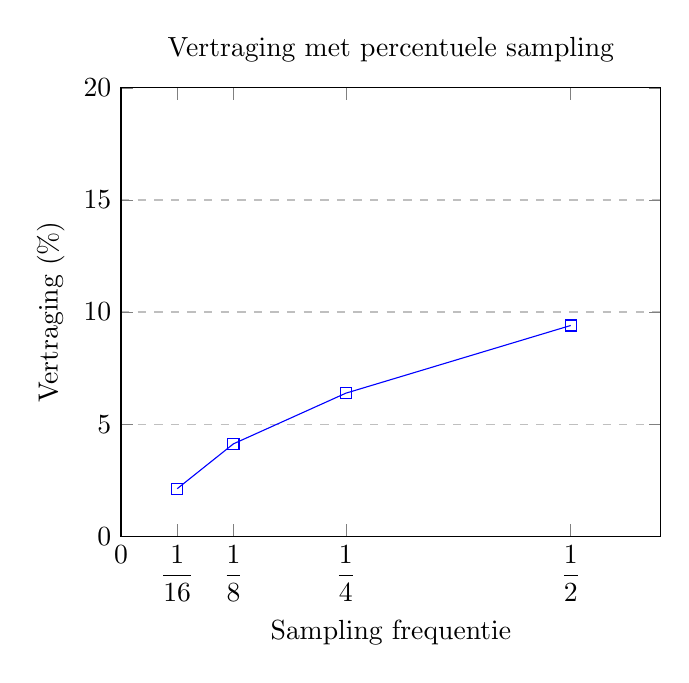
\begin{tikzpicture}
\begin{axis}[
    title={Vertraging met percentuele sampling},
    xlabel={Sampling frequentie},
    ylabel={Vertraging (\%)},
    xmin=0, xmax=0.6,
    ymin=0, ymax=20,
    xtick={0,0.0625,0.125,0.25,0.5},
    ytick={0,5,10,15,20},
    xticklabel style={/pgf/number format/.cd,frac,frac TeX=\displaystyle\frac},
    legend pos=north west,
    ymajorgrids=true,
    grid style=dashed,
    xlabel near ticks,
    ylabel near ticks
]
 
\addplot[
    color=blue,
    mark=square,
    ]
    coordinates {(0.0625,2.12)(0.125,4.12)(0.25,6.38)(0.5,9.4)};
 
\end{axis}
\end{tikzpicture}
\\\\

Verder wordt verwacht dat de visualisatie van tracing en logging de meerwaarde van Zipkin en Kibana zou schetsen en de voor- en nadelen van tracing aangetoond worden in verschillende situaties. \\

%---------- Verwachte conclusies ----------------------------------------------
\section{Verwachte conclusies}
\label{sec:verwachte_conclusies}

De verwachte conclusie is dat tracing onmisbaar is voor microservices en dit gestaafd is met uitgewerkte situaties in een opgestelde testomgeving. \\

%------------------------------------------------------------------------------
% Referentielijst
%------------------------------------------------------------------------------
% TODO: de gerefereerde werken moeten in BibTeX-bestand ``biblio.bib''
% voorkomen. Gebruik JabRef om je bibliografie bij te houden en vergeet niet
% om compatibiliteit met Biber/BibLaTeX aan te zetten (File > Switch to
% BibLaTeX mode)

\phantomsection
\printbibliography[heading=bibintoc]

\end{document}
